\subsection{Risikobewertung}

Die Risiken des Projektes sind gesammelt und bewertet worden. Pro Risiko wurden Massnahmen zur Prävention und zur Mitigation gesammelt. Die Bewertung wurde durchgeführt vor dem Umsetzen der Massnahmen (V.) und nachher (N.).
Zusätzlich zu den definierten Massnahmen sollen mithilfe von Prototypen so viele Risiken wie möglich, so gut wie möglich vermindert werden. 

Alle Risiken wurden bewertet anhand der Wahrscheinlichkeit und der Auswirkung. 
Die Risiken sind in den zwei Tabellen dargestellt, einmal vor dem Definieren der Massnahmen und einmal nach Umsetzung der definierten Massnahmen. Die Beschreibung aller Risiken befindet sich in der nachfolgenden Tabelle.


\begin{table}[H]
\begin{subtable}{0.5\textwidth}
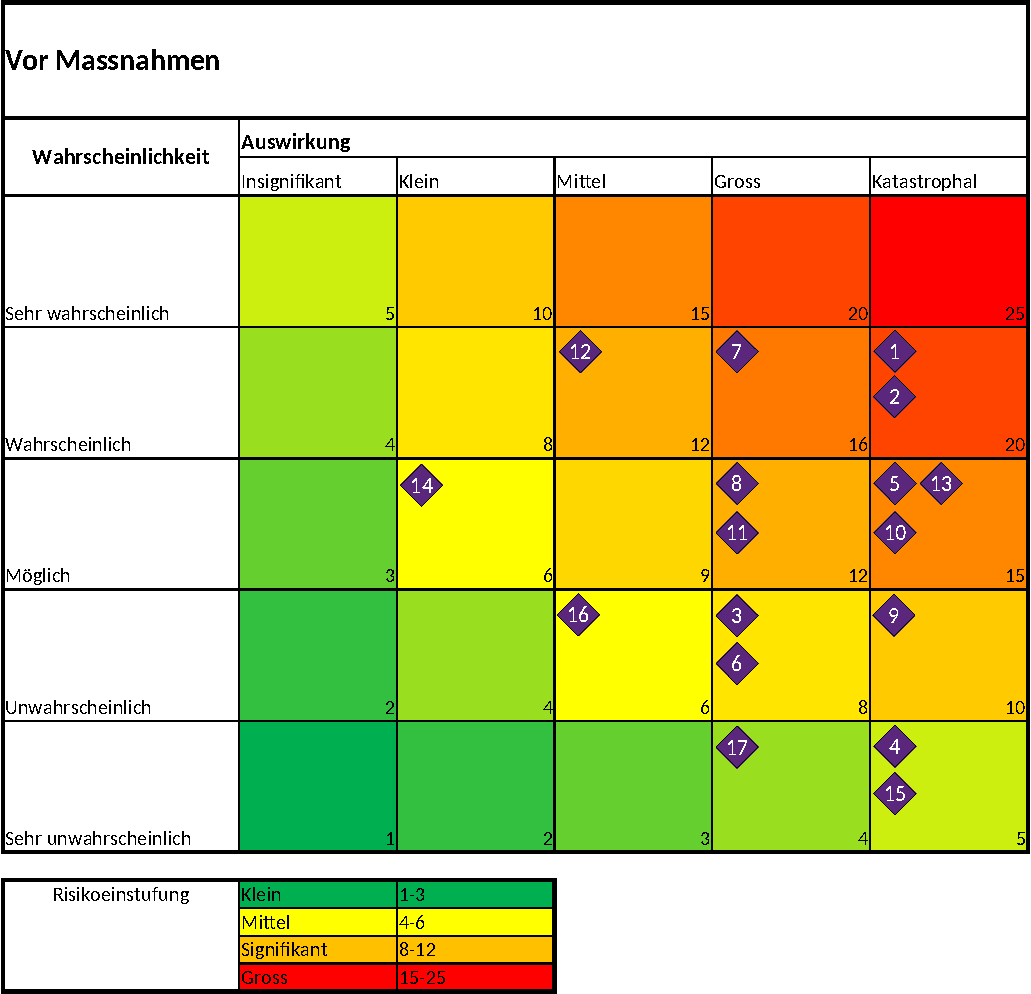
\includegraphics[width=0.99\linewidth]{assets/Risikoanalyse_vor_Massnahmen.pdf}
\caption{vor Massnahmen}
\label{table:risk-before}
\end{subtable}
\begin{subtable}{0.5\textwidth}
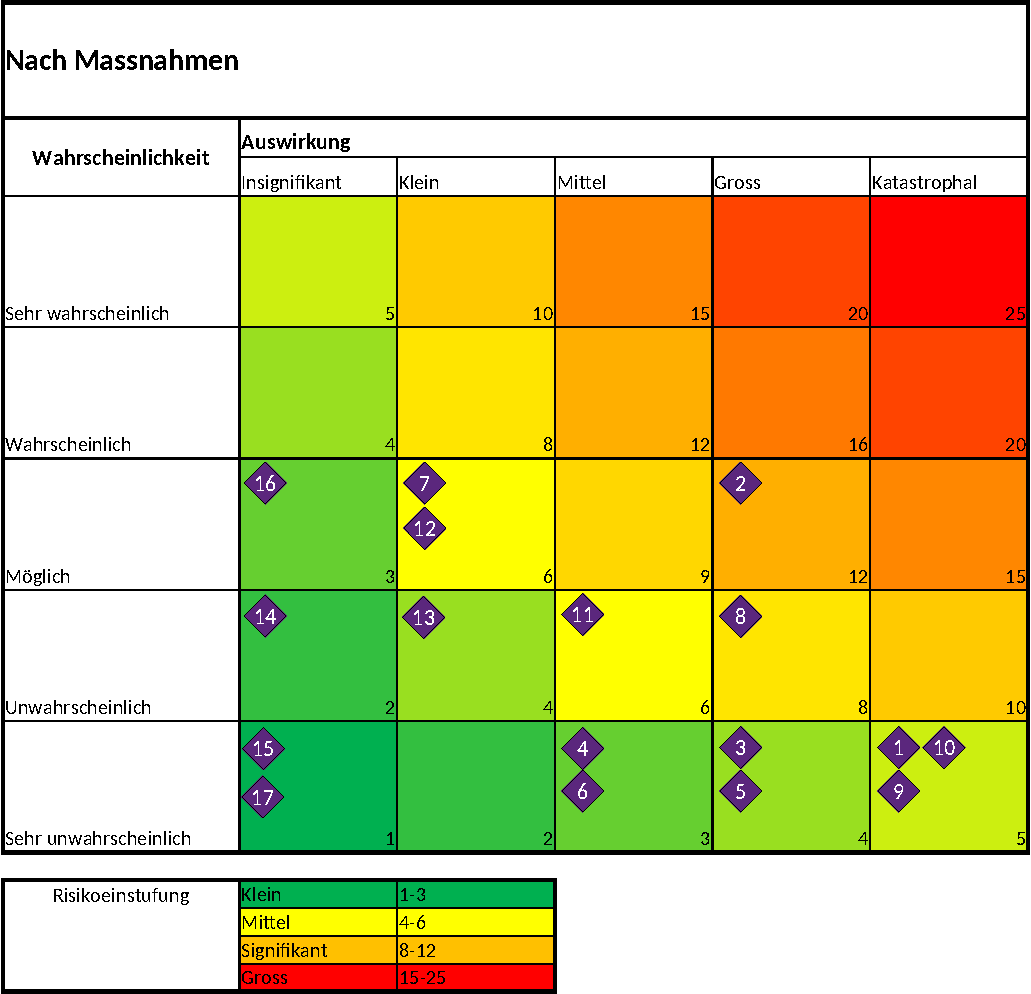
\includegraphics[width=0.99\linewidth]{assets/Risikoanalyse_nach_Massnahmen.pdf}
\caption{nach Massnahmen}
\label{table:risk-after}
\end{subtable}
\caption{Risikoanalyse}
\label{table:risk-table}
\end{table}

Aus der Risikomatrix nach den Massnahmen geht hervor, dass die grössten Risiken, die beim Entwickeln des Roboters berücksichtigt werden müssen, die folgenden drei sind:

\begin{itemize}
    \item Risiko 2: Knoten werden nicht erkannt.
    \item Risiko 7: Ein Objekt wird fehlerhaft gedeutet und falsche Wege werden intern entfernt.
    \item Risiko 12: Der Roboter wählt einen falschen Pfad, weil die Hinderniserkennung fehlerhaft ist.
\end{itemize}

Die folgende Tabelle zeigt alle Risiken detailliert auf.

\begin{table}[H]
\centering
\small
\begin{tabularx}\textwidth{|c | X | X | X | c | c|}
\hline
  \textbf{Nr} & \textbf{Beschreibung} & \textbf{Prävention} & \textbf{Mitigation} & \textbf{V.} & \textbf{N.} \\
  \hline
    1&Hindernisse werden nicht erkannt. &Mit vielen Bildern trainieren.& Distanzsensor; Roboter fährt zurück.&20&5 \\
  \hline
      2&Knoten werden nicht erkannt. &Viele Bilder in verschiedenen Situationen machen, um zu trainieren.&Linien werden erkannt und Roboter orientiert sich daran.&20& 12\\
  \hline
      3&4 Minuten reichen nicht. &Testdurchfläufe in realistischen Umgebungen.&&8&4 \\
  \hline
      4& 1 Minute reicht nicht zum Aufbau.& Testdurchfläufe und einfaches Interface.&Zufälliges Ziel wird gewählt von SW.&5&3 \\
  \hline
      5&Bodenfugen werden als Linie erkannt. & Testdurchfläufe in realistischen Umgebungen.&Kamera hilft Linien zu erkennen, hilft Roboter gerade zu stellen.&15&4 \\
  \hline
      6& Liniensensor fehlerhaft. &Sichere Implementation mit Tests.& Encoder Motoren.&8&3 \\
  \hline
      7& Ein Objekt wird fehlerhaft gedeutet und falsche Wege werden intern entfernt. &Knoten erkennen und nicht nur Hindernisse.&Roboter ist schnell genug und hat einen Trial \& Error Modus.&16&6 \\
  \hline
      8&Hindernisse werden beim Anheben verschoben. &Robuste Greifmethode wählen und testen.&&12&8 \\
  \hline
      9&Überstrom bei blockierten Motoren. &Endschalter, Stromsensoren.&Abschalten bevor Bauteile beschädigt.&10&5 \\
  \hline
      10&Ungenaue Abfahrtsituation vom Knoten, Fahrzeug fährt von der Linie weg. &Liniensensor als Unterstützung, Kamera prüft Linie&Korrigieren falls nötig.&15&5 \\
  \hline
      11&Die Kamera liefert unscharfe oder verzerrte unbrauchbare Bilder. &Verwendung von Kameras mit hoher Auflösung.&Falls Bilder unscharf sind, Roboter anhalten und neue Bilder aufnehmen.&12&6 \\
  \hline
      12& Der Roboter wählt einen falschen Pfad, weil die Hinderniserkennung fehlerhaft ist.&Optimierung der Hinderniserkennung.&Roboter bei Fehlverhalten anhalten und zurücksetzen in vorherigen Zustand. Roboter ist schnell.&12& 6\\
  \hline
      13&Ein Softwarefehler führt zu einem Absturz während der Laufzeit, wodurch der Roboter stoppt oder Fehlfunktionen aufweist. &Exception Handling und umfangreiche Tests unter verschiedenen Bedingungen.&Automatischer SW-Neustart, Wiederaufnahme des letzten bekannten Zustands.&15&4 \\
  \hline
      14&Ein Software-Update führt zu neuen Fehlern oder ist nicht kompatibel mit der aktuellen Hardware. &Gründliche Tests vor dem Rollout eines Updates.&Möglichkeit, schnell zur vorherigen stabilen Version zurückzukehren.&6&2 \\
  \hline
      15&Akkustand ist zu niedrig bei Start des Laufes. & Anzeige des Akkustandes. Leicht austauschbarer Akku. Akku aufladen.&Ein zweiter Akku, der voll aufgeladen ist.&5& 1\\
  \hline
      16&Personenausfall durch Krankheit oder Unfall. &&Stellvertretungen und virtuelle Kommunikation.&6& 3\\
  \hline
      17&Datenkorruption. &&Regelmässige Backups.&4& 1\\
  \hline



\end{tabularx}
\caption{Risiken}
\label{table:risks}
\end{table}


